% Choose one to switch between slides and handout
\documentclass[]{beamer}
%\documentclass[handout]{beamer}

% Video Meta Data
\title{Bitcoin, Blockchain and Cryptoassets}
\subtitle{History of Digital Money}
\author{Prof. Dr. Fabian Schär}
\institute{University of Basel}

% Config File
% Packages
\usepackage[utf8]{inputenc}
\usepackage{hyperref}
\usepackage{gitinfo2}
\usepackage{tikz}
\usepackage{amsmath}
\usepackage{bibentry}
\usepackage{xcolor}
\usepackage{colortbl} % Add colour to LaTeX tables
\usepackage{caption}
\usepackage[export]{adjustbox}
\usepackage{pgfplots} \pgfplotsset{compat = 1.17}

% Color Options
\definecolor{highlight}{rgb}{0.65,0.84,0.82}
\definecolor{focus}{rgb}{0.72, 0, 0}

% Beamer Template Options
\beamertemplatenavigationsymbolsempty
\setbeamertemplate{footline}[frame number]
\setbeamercolor{structure}{fg=black}
\setbeamercolor{footline}{fg=black}
\setbeamercolor{title}{fg=black}
\setbeamercolor{frametitle}{fg=black}
\setbeamercolor{item}{fg=black}
\setbeamercolor{}{fg=black}
\setbeamercolor{bibliography item}{fg=black}
\setbeamercolor*{bibliography entry title}{fg=black}
\setbeamertemplate{items}[square]
\setbeamertemplate{enumerate items}[default]
\captionsetup[figure]{labelfont={color=black},font={color=black}}
\captionsetup[table]{labelfont={color=black},font={color=black}}

\setbeamertemplate{bibliography item}{\insertbiblabel}

% Link Icon Command
\newcommand{\link}{%
    \tikz[x=1.2ex, y=1.2ex, baseline=-0.05ex]{%
        \begin{scope}[x=1ex, y=1ex]
            \clip (-0.1,-0.1)
                --++ (-0, 1.2)
                --++ (0.6, 0)
                --++ (0, -0.6)
                --++ (0.6, 0)
                --++ (0, -1);
            \path[draw,
                line width = 0.5,
                rounded corners=0.5]
                (0,0) rectangle (1,1);
        \end{scope}
        \path[draw, line width = 0.5] (0.5, 0.5)
            -- (1, 1);
        \path[draw, line width = 0.5] (0.6, 1)
            -- (1, 1) -- (1, 0.6);
        }
    }

% Read Git Data from Github Actions Workflow
% Defaults to gitinfo2 for local builds
\IfFileExists{gitInfo.txt}
	{\input{gitInfo.txt}}
	{
		\newcommand{\gitRelease}{(Local Release)}
		\newcommand{\gitSHA}{\gitHash}
		\newcommand{\gitDate}{\gitAuthorIsoDate}
	}

% Custom Titlepage
\defbeamertemplate*{title page}{customized}[1][]
{
  \vspace{-0cm}\hfill
\includegraphics[width=2.5cm]{../config/logo_cif}
  
\includegraphics[width=1.9cm]{../config/seal_wwz}
  \\ \vspace{2em}
  \usebeamerfont{title}\textbf{\inserttitle}\par
  \usebeamerfont{title}\usebeamercolor[fg]{title}\insertsubtitle\par  \vspace{1.5em}
  \small\usebeamerfont{author}\insertauthor\par
  \usebeamerfont{author}\insertinstitute\par \vspace{2em}
  \usebeamercolor[fg]{titlegraphic}\inserttitlegraphic
    \tiny \noindent \texttt{Release Ver.: \gitRelease}\\ 
    \texttt{Version Hash: \gitSHA}\\
    \texttt{Version Date: \gitDate}\\ \vspace{1em}
  \link \href{https://github.com/cifunibas/Bitcoin-Blockchain-Cryptoassets/blob/main/slides/intro.pdf}
  {Get most recent version}\\
  \link \href{https://github.com/cifunibas/Bitcoin-Blockchain-Cryptoassets/blob/main/slides/intro.pdf}
  {Watch video lecture}\\ \vspace{1em}
  License: \texttt{Creative Commons Attribution-NonCommercial-ShareAlike 4.0 International}\\\vspace{2em}
  
\includegraphics[width = 1.2cm]{../config/license}
}

% tikzlibraries
\usetikzlibrary{decorations.pathreplacing}
\usetikzlibrary{decorations.markings}
\usetikzlibrary{positioning}

%caption font
\captionsetup{font=footnotesize}


%%%%%%%%%%%%%%%%%%%%%%%%%%%%%%%%%%%%%%%%%%%%%%
%%%%%%%%%%%%%%%%%%%%%%%%%%%%%%%%%%%%%%%%%%%%%%
\begin{document}

\thispagestyle{empty}
\begin{frame}[noframenumbering]
	\titlepage
\end{frame}

%%%
\begin{frame}{Before Bitcoin}

\begin{figure}
	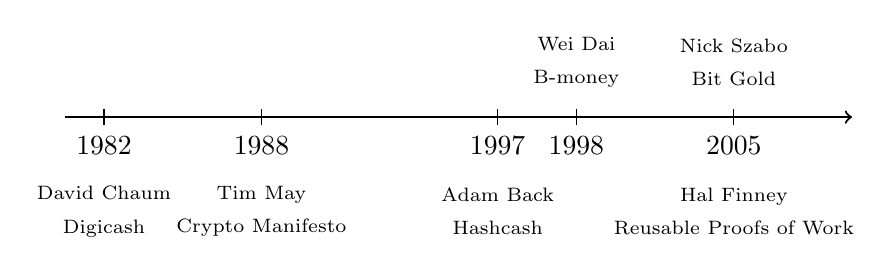
\begin{tikzpicture}[scale=1]
	
	%draw horizontal line
	\draw [thick,->] (0,0) -- (10,0);
	
	%draw vertical lines
	\foreach \x in {0.5,2.5,5.5,6.5,8.5}
	\draw (\x cm, 3pt) -- (\x cm, -3pt);
	
	%years
	\draw[ultra thick] (0.5,0) node[below=3pt] {1982} ;
	\draw[ultra thick] (2.5,0) node[below=3pt] {1988} ;
	\draw[ultra thick] (5.5,0) node[below=3pt] {1997} ;
	\draw[ultra thick] (6.5,0) node[below=3pt] {1998} ;
	\draw[ultra thick] (8.5,0) node[below=3pt] {2005} ;	
	
	%Text
	\node[align=center] at (0.5,-1.2) {{\scriptsize David Chaum} \\{\scriptsize Digicash}};
	
	\node[align=center] at (2.5,-1.2) {{\scriptsize Tim May} \\{\scriptsize Crypto Manifesto}};
	
	\node[align=center] at (5.5,-1.2) {{\scriptsize Adam Back} \\{\scriptsize Hashcash}};
	
	\node[align=center] at (6.5,0.7) {{\scriptsize Wei Dai} \\{\scriptsize B-money}};
	
	\node[align=center] at (8.5,-1.2) {{\scriptsize Hal Finney} \\{\scriptsize Reusable Proofs of Work}};
	
	\node[align=center] at (8.5,0.7) {{\scriptsize Nick Szabo} \\{\scriptsize Bit Gold}};
	
	\end{tikzpicture}
\end{figure}
\end{frame}
%%%


%%%
\begin{frame}{Digicash (1982) - David Chaum}
	\begin{itemize}
		\item Electronic means of payment would significantly limit privacy and traceable payment flows would generate sensitive data.
		\item Wanted to develop a virtual money unit that imitated the anonymity of cash.
		\item Monopolized money creation and centralized settlement.
		\item Central bank blindly signs money units.
	\end{itemize}
\end{frame}
%%%	


%%%
\begin{frame}{Hashcash (1997) - Adam Back}
	\begin{itemize}
		\item originally proposed as a mechanism for email anti-DoS.
		\item "I've been talking about a partial hash collision based postage scheme on the crypto lists for the last few days. The idea of using partial hashes is that they can be made arbitrarily expensive to compute (by choosing the desired number of bits of collision), and yet can be verified instantly."
	\end{itemize}
\end{frame}
%%%


%%%
\begin{frame}{B-money (1998) - Wei Dai}
	\begin{itemize}
		\item Thought experiment
		\item "I am fascinated by Tim May's crypto-anarchy."
		\item "\dots I will assume the existence of an untraceable network, where senders and receivers are identified only by digital pseudonyms (i.e. public keys) and every message is signed by its sender and encrypted to its receiver."
		\item " \dots every participant maintains a (separate) database of how much money belongs to each pseudonym. These accounts collectively define the ownership of money, and how these accounts are updated is the subject of this protocol."
	\end{itemize}
\end{frame}
%%%


%%%
\begin{frame}{Reusable Proofs of Work (2005) - Hal Finney}
	\begin{itemize}
		\item Combines ideas of Wei Dai and Adam Back
		\item "A PoW token is something that takes a relatively long time to compute but which can be checked quickly. RPoW uses hashcash, which are values whose SHA-1 hashes have many high bits of zeros."
	\end{itemize}
\end{frame}
%%%


%%%
\begin{frame}{Bit Gold (2005) - Nick Szabo}
	\begin{itemize}
		\item Describes the combination of the proof-of-work algorithm for competitive money creation.
		\item "Thus, it would be very nice if there were a protocol whereby unforgeably costly bits could be created online with minimal dependence on trusted third parties, and then securely stored, transferred, and assayed with similar minimal trust. Bit gold."
	\end{itemize}
\end{frame}
%%%


%%%
\begin{frame}{After Bitcoin: Forks and Altcoins}

\begin{figure}
	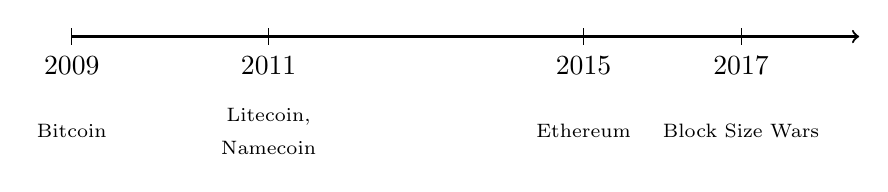
\begin{tikzpicture}[scale=1]
	
	%draw horizontal line
	\draw [thick,->] (0,0) -- (10,0);
	
	%draw vertical lines
	\foreach \x in {0,2.5,6.5,8.5}
	\draw (\x cm, 3pt) -- (\x cm, -3pt);
	
	%years
	\draw[ultra thick] (0,0) node[below=3pt] {2009} ;
	\draw[ultra thick] (2.5,0) node[below=3pt] {2011} ;
	\draw[ultra thick] (6.5,0) node[below=3pt] {2015} ;
	\draw[ultra thick] (8.5,0) node[below=3pt] {2017} ;
	
	
	
	%Text
	\node[align=center] at (0,-1.2) {{\scriptsize Bitcoin}};
	\node[align=center] at (2.5,-1.2) {{\scriptsize Litecoin,} \\{\scriptsize Namecoin}};
	\node[align=center] at (6.5,-1.2) {{\scriptsize Ethereum}};
	\node[align=center] at (8.5,-1.2) {{\scriptsize Block Size Wars}}; %\\{\scriptsize (Bitcoin Cash, SegWit,}\\{\scriptsize Bitcoin Gold, Bitcoin SV)}};
	

	
	\end{tikzpicture}
\end{figure}
\end{frame}
%%%


%%%%
\begin{frame}{Bitcoin Fork Timeline}
\begin{figure}[h!]
\center
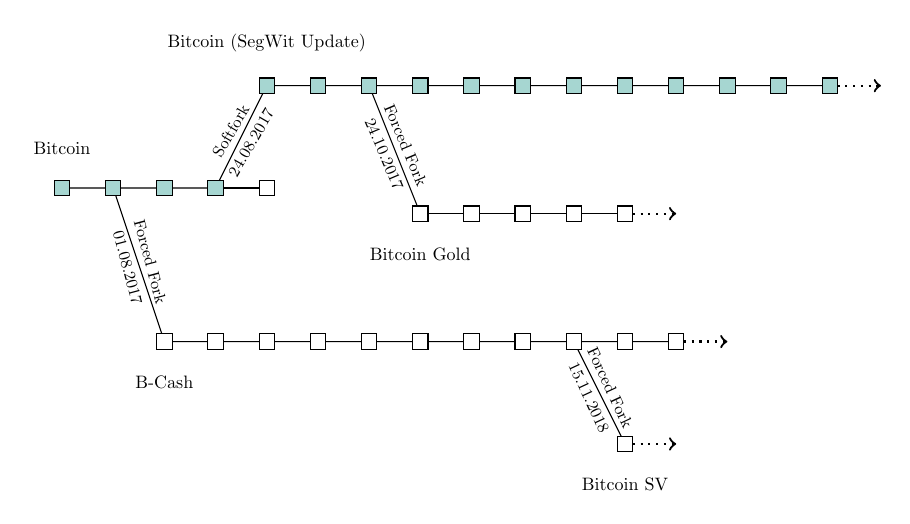
\begin{tikzpicture}[scale=0.65, every node/.style={scale=0.65}]

\coordinate (o1) at (1,1);
\coordinate (o2) at (2,1);
\coordinate (o3) at (3,1);
\coordinate (o4) at (4,1);
\coordinate (o5) at (5,3);
\coordinate (o6) at (6,3);
\coordinate (o7) at (7,3);
\coordinate (o8) at (8,3);
\coordinate (o9) at (9,3);
\coordinate (o10) at (10,3);
\coordinate (o11) at (11,3);
\coordinate (o12) at (12,3);
\coordinate (o13) at (13,3);
\coordinate (o14) at (14,3);
\coordinate (o15) at (15,3);
\coordinate (o16) at (16,3);
\coordinate (o17) at (17,3);
\coordinate (n1) at (3,-2);
\coordinate (n2) at (4,-2);
\coordinate (n3) at (5,-2);
\coordinate (n4) at (6,-2);
\coordinate (n5) at (7,-2);
\coordinate (n6) at (8,-2);
\coordinate (n7) at (9,-2);
\coordinate (n8) at (10,-2);
\coordinate (n9) at (11,-2);
\coordinate (n10) at (12,-2);
\coordinate (n11) at (13,-2);
\coordinate (n12) at (14,-2);
\coordinate (s2) at (12,-4);
\coordinate (s3) at (13,-4);
\coordinate (x5) at (5,1);
\coordinate (z1) at (8,0.5);
\coordinate (z2) at (9,0.5);
\coordinate (z3) at (10,0.5);
\coordinate (z4) at (11,0.5);
\coordinate (z5) at (12,0.5);
\coordinate (z6) at (13,0.5);

  \node at (o1) [above=1em]{Bitcoin};
  \node at (n1) [below=1em]{B-Cash};
  \node at (o5) [above=1em]{Bitcoin (SegWit Update)};
  \node at (z1) [below=1em]{Bitcoin Gold};
  \node at (s2) [below=1em]{Bitcoin SV};

  \draw[] (o1) to[] (o2) to[] (o3) to[] (o4) to[] node[below, rotate=60]{\small{24.08.2017}}node[above, rotate=60]{\small{Softfork}}  (o5) to[] (o6) to[] (o7) to[] (o8) to[] (o9) to[] (o10) to[] (o11) to[] (o12) to[] (o13) to[] (o14) to[] (o15) to[] (o16) ;
  \draw[] (o2) to[] node [above, rotate=-75]{\small Forced Fork} node[below, rotate=-75]{\small{01.08.2017}} (n1)  to[] (n2) to[] (n3) to[] (n4) to[] (n5) to[] (n6) to[] (n7) to[] (n8) to[] (n9) to[] (n10) to[] (n11);
  \draw[] (n9) to[] node [above, rotate=-65]{\small Forced Fork} node[below, rotate=-65]{\small{15.11.2018}} (s2) ;
  \draw[] (o4) to[] (x5) ;
  \draw[] (o7) to[] node [above, rotate=-67]{\small Forced Fork} node[below, rotate=-67]{\small{24.10.2017}} (z1) ;
  \draw[] (z1) to[] (z2) to[] (z3) to[] (z4) to[] (z5);
  %\draw[color=black] (n6) to[] (o7);
  %\draw[color=black,densely dashed] (o4) to[] (o5);
  %\draw[color=black,densely dashed] (o7) to[] (o8);
  \draw[color=black,thick, dotted, ->] (o16) to[] (o17);
  \draw[color=black,thick, dotted, ->] (n11) to[] (n12);
  \draw[color=black,thick, dotted, ->] (s2) to[] (s3);  
  \draw[color=black,thick, dotted, ->] (z5) to[] (z6);  

  %\filldraw[draw=black,fill=white] (o1) circle (5pt);
  %\filldraw[draw=black,fill=white] (o2) circle (5pt);
  %\filldraw[draw=black,fill=white] (o3) circle (5pt);
  %\filldraw[draw=black,fill=white] (o4) circle (5pt);
  %\filldraw[draw=black,fill=white] (o5) circle (5pt);
  %\filldraw[draw=black,fill=white] (o6) circle (5pt);
  %\filldraw[draw=black,fill=white] (o7) circle (5pt);
  %\filldraw[draw=black,fill=white] (o8) circle (5pt);
  %\filldraw[draw=black,fill=white] (o9) circle (5pt);
  \node (rect) at (o1) [fill=highlight,draw,minimum width=0.3cm,minimum height=0.3cm] {};
  \node (rect) at (o2) [fill=highlight,draw,minimum width=0.3cm,minimum height=0.3cm] {};
  \node (rect) at (o3) [fill=highlight,draw,minimum width=0.3cm,minimum height=0.3cm] {};
  \node (rect) at (o4) [fill=highlight,draw,minimum width=0.3cm,minimum height=0.3cm] {};
  \node (rect) at (o5) [fill=highlight,draw,minimum width=0.3cm,minimum height=0.3cm] {};
  \node (rect) at (o6) [fill=highlight,draw,minimum width=0.3cm,minimum height=0.3cm] {};
  \node (rect) at (o7) [fill=highlight,draw,minimum width=0.3cm,minimum height=0.3cm] {};
  \node (rect) at (o8) [fill=highlight,draw,minimum width=0.3cm,minimum height=0.3cm] {};
  \node (rect) at (o9) [fill=highlight,draw,minimum width=0.3cm,minimum height=0.3cm] {};
  \node (rect) at (o10) [fill=highlight,draw,minimum width=0.3cm,minimum height=0.3cm] {};
  \node (rect) at (o11) [fill=highlight,draw,minimum width=0.3cm,minimum height=0.3cm] {};
  \node (rect) at (o12) [fill=highlight,draw,minimum width=0.3cm,minimum height=0.3cm] {};
  \node (rect) at (o13) [fill=highlight,draw,minimum width=0.3cm,minimum height=0.3cm] {};
  \node (rect) at (o14) [fill=highlight,draw,minimum width=0.3cm,minimum height=0.3cm] {};
  \node (rect) at (o15) [fill=highlight,draw,minimum width=0.3cm,minimum height=0.3cm] {};
  \node (rect) at (o16) [fill=highlight,draw,minimum width=0.3cm,minimum height=0.3cm] {};
  %\filldraw[draw=black,fill=highlight] (n4) circle (5pt);
  %\filldraw[draw=black,fill=highlight] (n5) circle (5pt);
  %\filldraw[draw=black,fill=highlight] (n6) circle (5pt);
  %\filldraw[draw=black,fill=highlight] (n7) circle (5pt);
  %\filldraw[draw=black,fill=highlight] (n8) circle (5pt);
  %\filldraw[draw=black,fill=highlight] (n9) circle (5pt);
  \node (rect) at (n1) [fill=white,draw,minimum width=0.3cm,minimum height=0.3cm] {};
  \node (rect) at (n2) [fill=white,draw,minimum width=0.3cm,minimum height=0.3cm] {};
  \node (rect) at (n3) [fill=white,draw,minimum width=0.3cm,minimum height=0.3cm] {};
  \node (rect) at (n4) [fill=white,draw,minimum width=0.3cm,minimum height=0.3cm] {};
  \node (rect) at (n5) [fill=white,draw,minimum width=0.3cm,minimum height=0.3cm] {};
  \node (rect) at (n6) [fill=white,draw,minimum width=0.3cm,minimum height=0.3cm] {};
  \node (rect) at (n7) [fill=white,draw,minimum width=0.3cm,minimum height=0.3cm] {};
  \node (rect) at (n8) [fill=white,draw,minimum width=0.3cm,minimum height=0.3cm] {};
  \node (rect) at (n9) [fill=white,draw,minimum width=0.3cm,minimum height=0.3cm] {};
  \node (rect) at (n10) [fill=white,draw,minimum width=0.3cm,minimum height=0.3cm] {};
  \node (rect) at (n11) [fill=white,draw,minimum width=0.3cm,minimum height=0.3cm] {};
  %\node (rect) at (s1) [fill=white,draw,minimum width=0.3cm,minimum height=0.3cm] {};
  \node (rect) at (s2) [fill=white,draw,minimum width=0.3cm,minimum height=0.3cm] {};
  \node (rect) at (x5) [fill=white,draw,minimum width=0.3cm,minimum height=0.3cm] {};
  \node (rect) at (z1) [fill=white,draw,minimum width=0.3cm,minimum height=0.3cm] {};
  \node (rect) at (z2) [fill=white,draw,minimum width=0.3cm,minimum height=0.3cm] {};
  \node (rect) at (z3) [fill=white,draw,minimum width=0.3cm,minimum height=0.3cm] {};
  \node (rect) at (z4) [fill=white,draw,minimum width=0.3cm,minimum height=0.3cm] {};
  \node (rect) at (z5) [fill=white,draw,minimum width=0.3cm,minimum height=0.3cm] {};
  
\end{tikzpicture}
\caption{Bitcoin fork timeline.}
\label{fig:forkhistory}
\end{figure}

\end{frame}



\end{document}